\section{Radioactive Decay}
\begin{figure}[ht!]
\centering
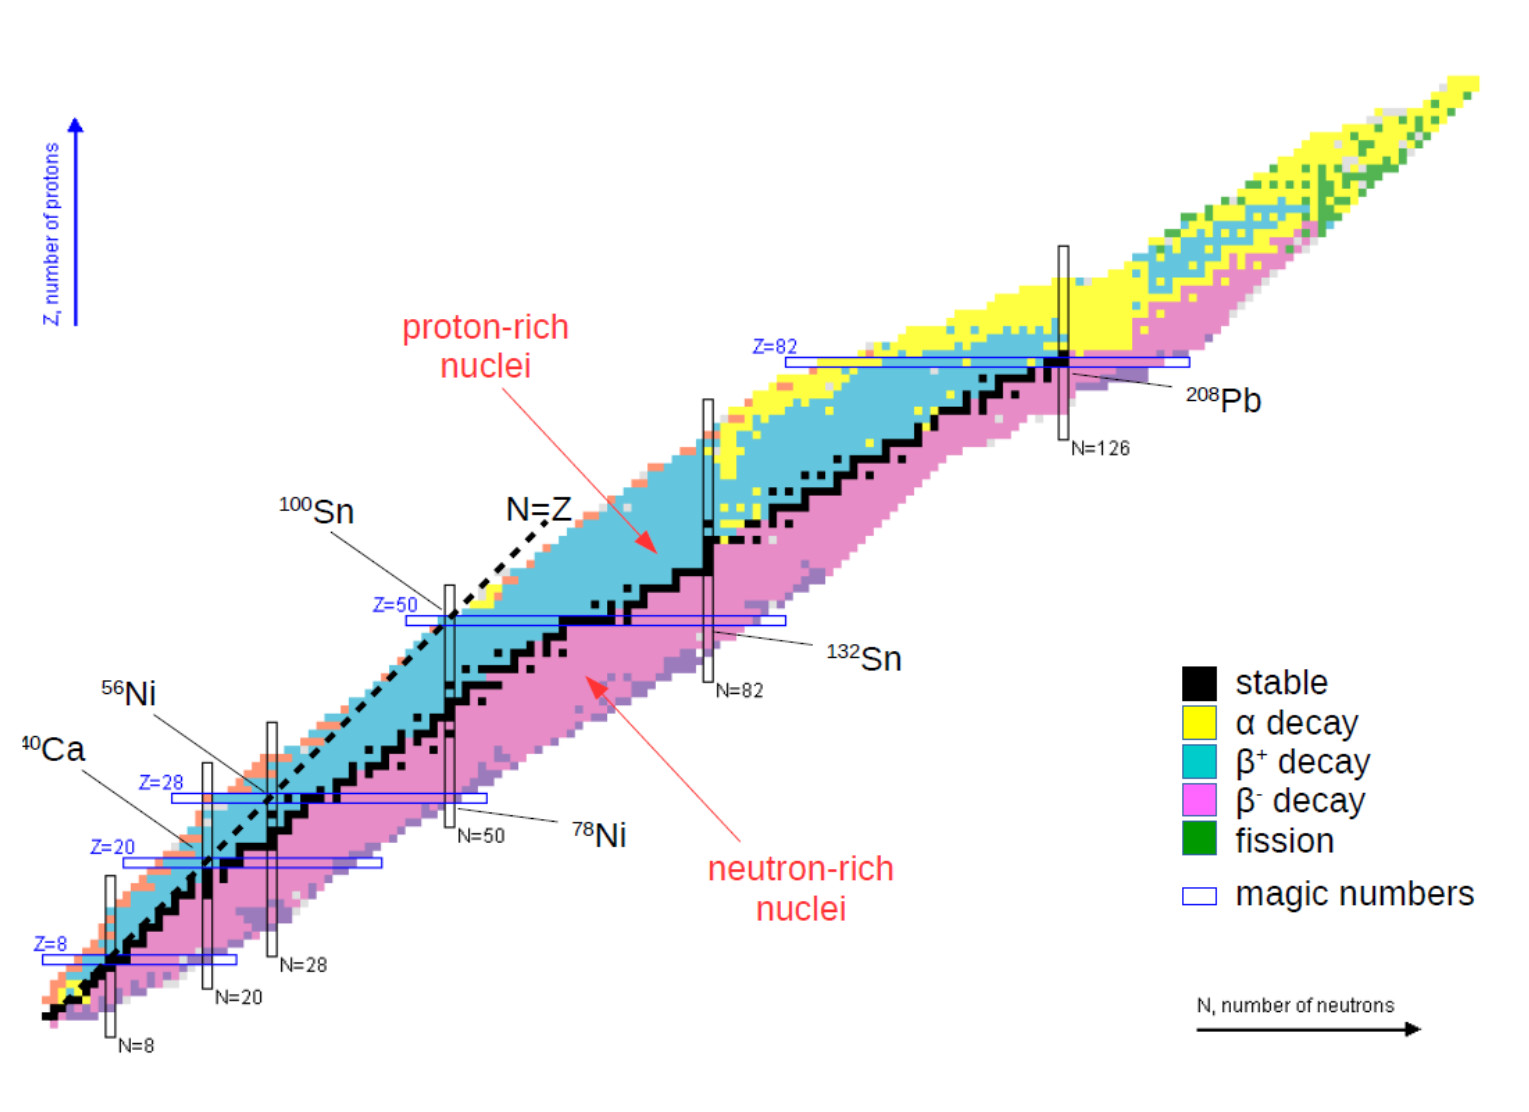
\includegraphics[width = .8\textwidth]{radioactive_nuclei_chart.png}
\caption{Chart of the nuclei and their decay modes.}
\label{fig: radioactive_nuclei_chart}
\end{figure}

\begin{itemize}
    \item Naturally occurring nuclei goes through a combination of $α$, $β$ and $γ$ decay.
    \item Spontaneous decays occur when the $Q$-value is positive 
    \begin{equation}
      Q = (M_i - M_f)c^2
    \end{equation}
    \item Artificially produced nuclei can also decay by spontaneous fission, neutron emission, proton emission and heavy iron emission in addition to the natural decay modes.
\end{itemize}

\subsection{Exponential Decay}
\subsubsection{The Law}
The number of radioactive nuclei $N(t)$ at time $t$ is given by the exponential decay law, where $λ$ is the decay constant. 
\begin{equation}
  N(t) = N_0 e^{-λt}
\end{equation}

\subsubsection{Half-Life}
The time it takes to reduce the intensity of radiation by half. 
\begin{equation}
  t_{1/2} = \frac{\ln 2}{λ} ≈ \frac{0.693}{λ}
\end{equation}

\subsubsection{Mean Lifetime}
The average time that a  nucleus is likely to survive before decaying. This is often referred to as the lifetime of the nucleus.
\begin{equation}
  τ = \frac{1}{λ}
\end{equation}

\subsubsection{Activity}
Activity is the number of decays per unit time. This is a lot more practical to work with, as it is easier to measure the number of decays in a given time period than the number of nuclei.
\begin{equation}
  A(t) = \frac{\mathrm{d}N(t)}{\mathrm{d}t} =  A_0 e^{-λt} \quad , \quad  A_0 = λN_0
\end{equation}

\paragraph{Units of Activity:} 
The unit of activity is the Becquerel (Bq). 
\begin{equation}
  1 \text{ Bq} = 1 \text{ decay/s}
\end{equation}
It is more common to use the Curie (Ci). 1 Ci i the activity of 1g of $\ce{_{}^{226}\text{Ra}_{}}$
\begin{equation}
  1 \text{ Ci} = 3.7 \times 10^{10} \text{ Bq}
\end{equation}

\paragraph{Important Note:}
Knowing the activity, does not tell you its lifetime or halflife and vice versa. Saying something is highly radioactive, does not tell you about the danger or the energy of the radiation.

\subsubsection{Measuring Short and Long Lifetimes and Activity}
\begin{itemize}
    \item After 10 half-lives, the activity is reduced to $1/1024$ of the original activity. We assume the activity is zero after 10 half-lives. 
    \item This means if the half-lifte is short (like 1 second), you have only 10 seconds to measure the activity.
    \item If the half life is very long (like 100 years), you will not live to measure the activity.
\end{itemize}

\subsubsection{When the Decay Law Fails}
If the parent nucleus decays into a daughter nucleus, which is also radioactive, the decay law fails as the number of children does not stay the same, they create grandchildren. 

\subsection{Decay Options}  
For isotopes which are able to decay in multiple ways, the total decay rate is the sum of the decay rates for each decay mode.
\begin{equation}
  λ_\text{tot} = ∑_{i}^{} λ_i = \frac{1}{τ_\text{tot}} = ∑_{i}^{} \frac{1}{τ_i}
\end{equation}

\subsection{Mixed Samples}
\begin{wrapfigure}{r}{0.4\textwidth}
\vspace{-6.5mm}
\centering
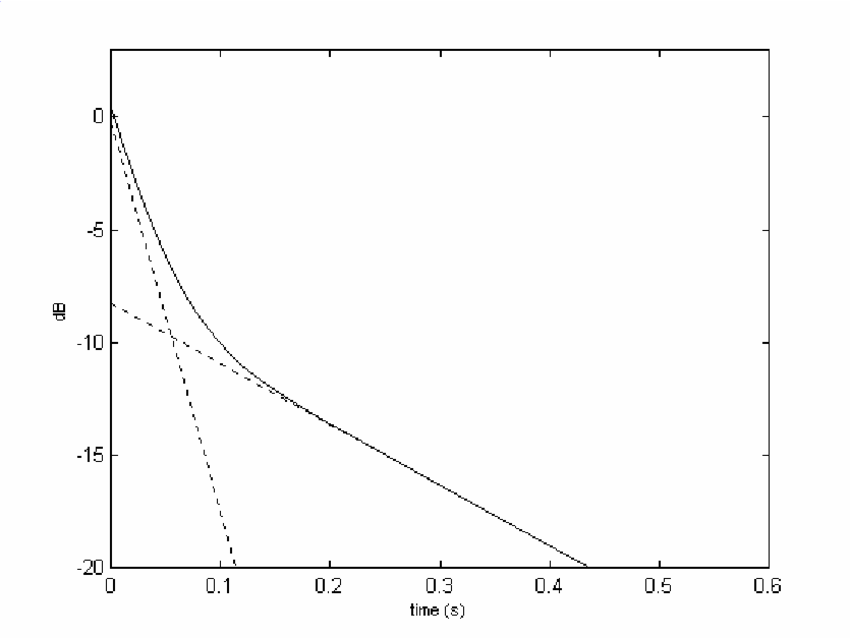
\includegraphics[width = .35\textwidth]{mixed_sample_decay.png}
\caption{Visualisation of the decay of a mixed sample. The y-axix is logarithmic.}
\label{fig: mixed_sample_decay}
\end{wrapfigure}
With more than one isotope in a sample, we can wait ten half-lives for the shortest lived isotope to decay, and then measure the activity of the remaining isotopes. This is the case for $\ce{}^{64}\text{Cu}_{}(12\text{h})$ and $\ce{}^{61}\text{Cu}_{}(3.4\text{h})$, which can't be separated chemically. Plotted out on a semi-log curve, we would still set a total decay curve looking logarithmic. If you wait until it becomes linear, you know you only have the decay of one isotope left. This is visualized in \cref{fig: mixed_sample_decay}.

\subsection{Types of Radioactive Decay}
\paragraph{$α$-Decay:}
Decaying of alpha particles ($\ce{_{}^{4}\text{H}_{}}$). This occurs when Radium decays to Radon. This has a half-life of about 1600 years.

\paragraph{$β$-Decay:} 
Split into two types, $β^-$ and $β^+$ decay. We also have electron capture.
\begin{itemize}
    \item $β^-$-Decay: A neutron decays into a proton, an electron and an electron antineutrino. This happens when $\ce{_{53}^{131}\text{I}_{78}}$ decays into $\ce{_{54}^{131}\text{Xe}_{77}}$. The half-life of which is 8 days.
    \item $β^+$-Decay: A proton decays into a neutron, a positron and an electron neutrino. A lone proton cannot decay, but a proton in a nucleus can. The half-life of a proton is $10^{34}$ years. An example ishw ne $\ce{_{13}^{25}\text{Al}_{12}}$ decays to $\ce{_{12}^{25}\text{Mg}_{13}}$, with a half-life of 7.2 seconds. 
    \item Electron Capture: A proton captures an electron and decays into a neutron and an electron-neutrino. An example is when $\ce{_{25}^{54}\text{Mn}_{29}}$ decays into $\ce{_{24}^{54}\text{Cr}_{30}}$ with a half-life of 312 days. Electron capture is more common in proton-rich nuclei with higher chance of $β^{+}$-decay. 
\end{itemize}

\paragraph{$γ$-Decay:}
When a nucleus is in an excited state, it can decay to a lower energy state by emitting a photon. The half-life can be anything from $1μ$s to minutes, to hours or even years. These are often called metastable states. Metastable states are noted with an $m$ like so: $\ce{_{Z}^{Am}\text{X}_{N}}$. For nuclear physics, one can consider nano-second half-lives as metastable. 


\subsubsection{Branching Ratios and Partial Half-Lives}
\begin{wrapfigure}{r}{0.5\textwidth}
\vspace{-4mm}
\centering
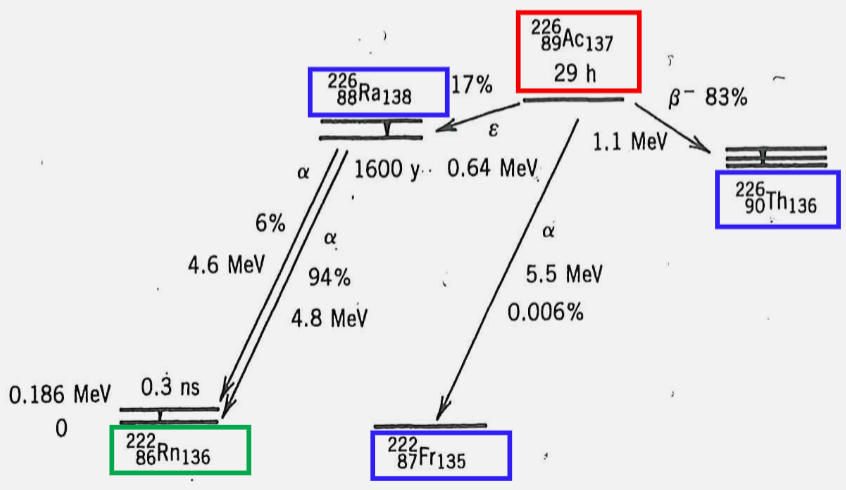
\includegraphics[width = .45\textwidth]{decay_branches.png}
\caption{Example of a parent (red) decaying into three different children (blue) by different modes. One of the children decays again into a grandchild (green).}
\label{fig: decay_branches}
\end{wrapfigure}
When a nucleus can decay in multiple ways, we get different branching ratios. The branching ratio is the fraction of decays that go through a specific decay mode. This is often referred to as the intensity of the decay modes. An example can be seen in \cref{fig: decay_branches}. 

To find the total half-life, we first use the total decay constant $λ_\text{tot}$, and then we can find the partial half-lives by. 
\begin{equation}
  λ_{\text{tot}} = \ln 2 / t_{1/2} ≈ 6.6 ⋅ 10^6 \text{s}^{-1}
\end{equation}
From this we find each decay constant as follows:
\begin{align}
  &λ_{β} = 0.83 λ_{\text{tot}}  = 5.5 ⋅ 10^6 \text{s}^{-1} \\
  &λ_{ε} = 0.17 λ_{\text{tot}}  = 1.1 ⋅ 10^6 \text{s}^{-1} \\
  &λ_{α} = 6 ⋅ 10^{-5} λ_{\text{tot}}  = 4.0 ⋅ 10^{-10} \text{s}^{-1}
\end{align}


And from here we easily find the partial half-lives.  
\begin{align}
  &t_{1/2,β} = \ln 2 / λ_{β} ≈ 1.3 ⋅ 10^{5} \text{s} ≈ 35 \text{h} \\
  &t_{1/2,ε} = \ln 2 / λ_{ε} ≈ 6.1 ⋅ 10^{5} \text{s} ≈ 170 \text{h} \\
  &t_{1/2,α} = \ln 2 / λ_{α} ≈ 1.7 ⋅ 10^{9} \text{s} ≈ 55 \text{y}
\end{align}
\subsubsection{Width-Lifetime Relation}
\paragraph{Stationary State:}
Does not decay. The energy is precisely defined with zero uncertainty. 
\begin{equation}
  ΔE = \sqrt{\langle E^2 \rangle - \langle E \rangle^2} = 0
\end{equation}
\begin{equation}
  ΔE Δt ≥ \frac{\hbar}{2}
\end{equation}

\paragraph{Non-Stationary State:}
Does eventually decay. The energy is not precisely defined, and has a finite uncertainty. A short lifetime means large decay and energy width, and vice versa. 
\begin{equation}
  ΔE = \sqrt{\langle E^2 \rangle - \langle E \rangle^2} ≠ 0
\end{equation}
\begin{equation}
  ΔE Δt ≥ \frac{\hbar}{2}
\end{equation}
\begin{equation}
  ΔE = Γ \quad , \quad  Δt = τ
\end{equation}
\begin{equation}
  τ ≈ \frac{\hbar}{Γ} = \frac{1}{λ}
\end{equation}